% Template para Proposta e TCC da EST/UEA -
% Padrão para os cursos do Núcleo de Computação
%
% Elaborado por Elloá B. Guedes
% Adaptado da versão elaborada por:
%                   Jucimar Maia Jr.
%
% Versão 1.3 - 15 de julho de 2022
%

\documentclass[a4paper,twoside,titlepage,12pt]{report}


\usepackage[utf8]{inputenc}
\usepackage[OT1]{fontenc}
\usepackage{ae}
\usepackage[brazil]{babel}
\usepackage{a4wide}
\usepackage{comment}
\usepackage[pdftex]{graphicx,color}
\usepackage{graphics}
\usepackage{cite}
\usepackage{longtable}
\usepackage{float}
\usepackage{fancyvrb}
\usepackage{fancyhdr}
\usepackage{setspace}
\usepackage{amsmath}
\usepackage{lscape}
\usepackage{textcase}
\usepackage{anysize}
\usepackage{setspace}
\usepackage{booktabs}
\usepackage{url}
\usepackage{subfig}
\usepackage{cite}
\usepackage[alf]{abntex2cite}
\usepackage{pdfpages}

\marginsize{20mm}{20mm}{20mm}{15mm}


%% Cabeçalhos
\renewcommand{\topfraction}{1}
\renewcommand{\bottomfraction}{1}
\renewcommand{\floatpagefraction}{1}
\renewcommand{\textfraction}{0}
%\renewcommand{\baselinestretch}{2}
\doublespacing %espaçamento duplo
\sloppy

%% Nomes
\floatstyle{plain}  %%% tipos: plain, boxed, ruled
\newfloat{codigo}{tbp}{lop}[section]
\floatname{codigo}{Código}

%%% nome para ser usado no sumário

\newcommand{\listofcodename}{Lista de C\'{o}digos}



% RESUMO ----------------------------------------------------------------------------------------------------------------------------------------------------------------------

\newcommand{\resumo}[1]{
\begin{center} \LARGE \bf Resumo \end{center}

\vskip 4em
\input{#1}

\newpage

}

% ABSTRACT ----------------------------------------------------------------------------------------------------------------------------------------------------------------------

\newcommand{\abstractt}[1]{
\begin{center} \LARGE \bf Abstract \end{center}

\vskip 4em
\input{#1}

\newpage

}

% Sumário -----------
\newcommand{\sumario}{
\renewcommand{\contentsname}{Sum\'{a}rio}
\tableofcontents
\addcontentsline{toc}{chapter}{\listtablename}
\listoftables

\newpage
\addcontentsline{toc}{chapter}{\listfigurename}
\listoffigures
\addcontentsline{toc}{chapter}{\listofcodename}
\listof{codigo}{\listofcodename}  % Lista de Códigos

\clearpage
}

\pagestyle{plain}

\newcommand{\folhaRosto}[5]{

\thispagestyle{empty}
\begin{center}
\textbf{\\[0.4em]\MakeUppercase{#2} \\[5cm]}
\textbf{\MakeUppercase{#1}\\[96pt]}

\end{center}

\hspace*{8cm}
\begin{minipage}{8cm}
Trabalho de Conclus\~{a}o de Curso
apresentado \`{a} banca avaliadora do Curso de Engenharia de Computa\c{c}\~{a}o, da
Escola Superior de Tecnologia, da Universidade do Estado do Amazonas, como
pr\'e-requisito para obten\c{c}\~{a}o do t\'{\i}tulo de Engenheiro de Computa\c{c}\~{a}o.\\[40pt]
\end{minipage}

\begin{center}
Orientador(a): #3 \\[12ex]
Manaus -- #4 -- #5\\
\end{center}


\pagenumbering{roman}
\newpage
}




%% Preencha aqui os seguintes dados
\def \titulo{Validação de Prescrição Médica com Inteligência Artificial Generativa: Análise de Interações Medicamentosas Baseada em Bula}
\def \orientador{Prof. Dr. Raimundo Corrêa de Oliveira}
\def \nome{George Lucas Lopes da Silva Gomes}
\def \mes{Março}
\def \ano{2025}

\begin{document}

\folhaRosto{\titulo}{\nome}{\orientador}{\mes}{\ano}

% Edite os seguintes arquivos para alterar as informações necessárias
\begin{center} \LARGE \bf Ficha Catalográfica \end{center}


\begin{enumerate}
    \item Estas instruções \textbf{não} devem ser entregues aos avaliadores do trabalho nas ocasiões dos TCCs 1 e 2. Portanto, comente a linha que importa este arquivo;
    \item A ficha catalográfica deve ser elaborada após a defesa do TCC2, quando você concluir as correções sugeridas pela banca e validar a versão final com o/a professor(a) orientador(a);
    \item Acessar \url{http://repositorioinstitucional.uea.edu.br:8080/ficha/ficha_catalografica.php} e preencher as informações requeridas para elaborar a ficha catalográfica;
    \item Incluir o pdf gerado na subpasta \emph{source} com o nome \texttt{ficha.pdf};
    \item Apagar todo o conteúdo deste arquivo e deixar apenas o comando a seguir:
    \begin{verbatim}
        \includepdf[pages=-]{./source/ficha.pdf}
    \end{verbatim}
\end{enumerate}

\newpage

\begin{center} \LARGE \bf Folha de Aprovação \end{center}


\begin{enumerate}
    \item Estas instruções \textbf{não} devem ser entregues aos avaliadores do trabalho nas ocasiões dos TCCs 1 e 2. Portanto, comente a linha que importa este arquivo;
    \item Após a defesa do TCC2, efetue as correções indicadas pela banca;
    \item Valide a versão final do trabalho com seu/sua orientador(a). Ele/Ela irá entregar uma carta de anuência ao coordenador da disciplina de TCC2 indicando estar de acordo com a versão final produzida;
    \item O responsável pela disciplina de TCC2 irá lhe entregar digitalmente um documento PDF com as assinaturas e aprovação dos integrantes da banca;
    \item O referido arquivo deve ser adicionado na pasta source com o nome \texttt{assinaturas.pdf};
    \item Todo o conteúdo deste arquivo deve ser retirado e substituído pelo seguinte comando:

   \begin{verbatim}
       \includepdf[pages=-]{./source/assinaturas.pdf}
   \end{verbatim}
\end{enumerate}

\newpage



% Indique onde esta o arquivo do resumo
\resumo{./files/resumo.tex}
% Idem para o abstract
\abstractt{./files/abstract.tex}


\sumario

% Configuração de cabeçalhos
\pagestyle{fancy}
\renewcommand{\chaptermark}[1]{\markboth{#1}{}}
\renewcommand{\sectionmark}[1]{\markright{#1}}
\renewcommand{\headrulewidth}{0.5pt}
\newcommand{\rom}{\fontfamily{cmr}\fontseries{m}\fontsize{10}{12}\selectfont}
\fancyhf{} \fancyhead[LE,RO]{\rom\thepage}
\fancyhead[LO]{\rom\rightmark} \fancyhead[RE]{\rom\leftmark}
\fancypagestyle{plain}{
    \fancyhead{} % get rid of headers
    \renewcommand{\headrulewidth}{0pt} % and the line
 }


\pagenumbering{arabic}



% Seus capítulos vão aqui --------
\chapter{Introdução}

\section{Justificativa}

A prescrição de medicamentos é uma prática essencial na área da saúde, mas erros de prescrição podem levar a complicações médicas graves, incluindo interações medicamentosas prejudiciais, reações adversas e falhas terapêuticas. Médicos e farmacêuticos enfrentam desafios diários ao garantir que uma prescrição seja segura e eficaz para o paciente, considerando variáveis como idade, peso, condições clínicas, alergias e medicamentos em uso.

A tecnologia pode desempenhar um papel fundamental na redução desses erros, proporcionando ferramentas inteligentes para análise e validação de prescrições. A aplicação proposta utilizará inteligência artificial e processamento de linguagem natural para analisar bulas de medicamentos em conjunto com os dados do paciente, gerando alertas automáticos sobre possíveis incompatibilidades.

Ao desenvolver essa solução, buscamos contribuir para a segurança do paciente, reduzir a carga de trabalho dos profissionais de saúde e oferecer uma ferramenta de suporte à decisão baseada em evidências.

\section{Objetivo Geral}

Desenvolver uma aplicação baseada em inteligência artificial que auxilie médicos e farmacêuticos na validação de prescrições médicas, analisando bulas de medicamentos e dados clínicos do paciente para identificar possíveis interações medicamentosas e alertar sobre incompatibilidades.

\section{Objetivos Específicos}

\begin{itemize}
    \item Criar um crawler para obter automaticamente bulas de medicamentos do site da Anvisa.
    \item Permitir upload e armazenamento de bulas, tanto as baixadas da Anvisa quanto as enviadas pelo usuário.
    \item Implementar um sistema de cadastro de pacientes, permitindo a inserção de informações médicas relevantes (idade, peso, histórico de doenças, alergias, medicamentos em uso, exames laboratoriais, etc.).
    \item Desenvolver um mecanismo de análise semântica das bulas utilizando Langchain.js e Elasticsearch para embeddings.
    \item Criar um mecanismo de análise automática de interações medicamentosas, validando prescrições médicas com base nos dados do paciente.
    \item Implementar alertas e recomendações baseadas em inteligência artificial, fornecendo insights para médicos e farmacêuticos no momento da prescrição.
\end{itemize}

\section{Metodologia}

\subsection{Desenvolvimento do Sistema}

O projeto será desenvolvido utilizando uma arquitetura modular, dividida nos seguintes componentes principais:

\begin{itemize}
    \item \textbf{Backend (NestJS + Prisma + PostgreSQL)}
    \begin{itemize}
        \item CRUD para cadastro de pacientes (nome, idade, peso, histórico clínico, alergias, medicamentos em uso).
        \item CRUD para cadastro de medicamentos e prescrições.
        \item Integração com MinIO para armazenamento de documentos médicos.
        \item API para comunicação com o frontend e com o módulo de inteligência artificial.
    \end{itemize}

    \item \textbf{Inteligência Artificial (Langchain.js + Elasticsearch)}
    \begin{itemize}
        \item Extração de informações de bulas de medicamentos.
        \item Indexação e busca semântica utilizando embeddings de IA.
        \item Geração de relatórios e validações por meio do modelo Claude Sonnet 3.5.
        \item Sugestões de ajustes nas prescrições médicas.
    \end{itemize}

    \item \textbf{Frontend (AngularJS + MaterialUI/Bootstrap)}
    \begin{itemize}
        \item Tela de cadastro de paciente.
        \item Interface para upload de documentos e pesquisa de bulas.
        \item Visualização de alertas e recomendações personalizadas.
    \end{itemize}
\end{itemize}

\section{Etapas do Projeto}

O desenvolvimento será dividido em sete etapas, cada uma com suas atividades e entregáveis.

\subsection{Etapa 1: Criar o Crawler da Anvisa}

\textbf{Objetivo:} Obter bulas de medicamentos automaticamente do site da Anvisa.

\textbf{Tarefas:}
\begin{itemize}
    \item Identificar as URLs relevantes e a estrutura do site da Anvisa.
    \item Definir a tecnologia do crawler (Scrapy, BeautifulSoup ou Selenium).
    \item Implementar o script para buscar e baixar bulas automaticamente.
    \item Criar uma base de metadados para armazenar informações extraídas.
    \item Lidar com possíveis bloqueios (CAPTCHA, rate limits).
\end{itemize}

\textbf{Previsão:} 1-2 semanas

\subsection{Etapa 2: Upload e Armazenamento de Arquivos}

\textbf{Objetivo:} Criar um sistema para armazenar bulas baixadas e arquivos enviados pelo usuário.

\textbf{Tarefas:}
\begin{itemize}
    \item Criar endpoints no backend (NestJS) para upload e consulta de arquivos.
    \item Configurar MinIO para armazenar documentos.
    \item Estruturar um banco de dados (PostgreSQL) para associar bulas aos usuários.
    \item Criar mecanismos para recuperação e listagem de arquivos.
\end{itemize}

\textbf{Previsão:} 1-2 semanas

\subsection{Etapa 3: Embeddings das Bulas}

\textbf{Objetivo:} Processar documentos para permitir consultas semânticas via IA.

\textbf{Tarefas:}
\begin{itemize}
    \item Criar um pipeline de processamento utilizando Langchain.js e Elasticsearch.
    \item Indexar bulas automaticamente para permitir pesquisa inteligente.
    \item Criar endpoints para busca por similaridade.
\end{itemize}

\textbf{Previsão:} 1 semana

\subsection{Etapa 4: Cadastro de Usuários}

\textbf{Objetivo:} Criar um sistema para cadastrar médicos e permitir autenticação.

\textbf{Tarefas:}
\begin{itemize}
    \item Criar a estrutura de usuários no PostgreSQL.
    \item Implementar autenticação JWT e gerenciamento de permissões.
    \item Criar interface de login e perfil no frontend.
\end{itemize}

\textbf{Previsão:} 1 semana

\subsection{Etapa 5: Upload de Arquivos de Usuários}

\textbf{Objetivo:} Permitir que médicos adicionem documentos médicos dos pacientes.

\textbf{Tarefas:}
\begin{itemize}
    \item Criar endpoints no backend para upload e armazenamento de arquivos.
    \item Associar documentos a pacientes no banco de dados.
    \item Criar a interface de gerenciamento de arquivos no frontend.
\end{itemize}

\textbf{Previsão:} 1-2 semanas

\subsection{Etapa 6: Embeddings dos Documentos do Usuário}

\textbf{Objetivo:} Permitir consultas inteligentes nos documentos médicos do paciente.

\textbf{Tarefas:}
\begin{itemize}
    \item Criar um pipeline de embeddings para os arquivos médicos.
    \item Indexar automaticamente os documentos ao serem enviados.
    \item Criar endpoints para busca semântica nos arquivos médicos.
\end{itemize}

\textbf{Previsão:} 1 semana

\subsection{Etapa 7: Análise de Interações Medicamentosas e Validação de Prescrição}

\textbf{Objetivo:} Criar alertas automáticos para identificar interações medicamentosas e validar prescrições.

\textbf{Tarefas:}
\begin{itemize}
    \item Criar prompts específicos para o Claude Sonnet 3.5 gerar relatórios.
    \item Implementar endpoints no backend para validação de interações medicamentosas.
    \item Criar uma interface no frontend para exibir os alertas ao médico.
\end{itemize}

\textbf{Previsão:} 2 semanas

\section{Próximo Passo}

Com base nesse planejamento, o primeiro passo será a implementação do crawler para obter bulas do site da Anvisa.
\chapter{Fundamentação Teórica}

\section{Inteligência Artificial}

A \textbf{Inteligência Artificial} (IA) é um campo da ciência da computação que busca desenvolver sistemas capazes de simular a capacidade humana de raciocínio, aprendizado e tomada de decisões \cite{russell2016artificial}. A IA é amplamente utilizada em diversas áreas, como reconhecimento de padrões, processamento de linguagem natural, automação de tarefas e suporte à decisão médica.

Dentre as técnicas de IA, destacam-se os algoritmos de aprendizado de máquina (\textit{Machine Learning}) e aprendizado profundo (\textit{Deep Learning}), que permitem aos sistemas aprenderem a partir de grandes volumes de dados e aprimorarem seu desempenho ao longo do tempo \cite{goodfellow2016deep}.

\section{Inteligência Artificial Generativa}

A \textbf{Inteligência Artificial Generativa} (\textit{Generative AI}) refere-se a uma classe de algoritmos de IA capazes de criar novos conteúdos a partir de exemplos previamente aprendidos. Esses modelos são frequentemente baseados em redes neurais profundas, como \textit{transformers}, \textit{autoencoders} variacionais (VAE) e redes adversárias generativas (GANs) \cite{brown2020language}.

Na área da saúde, modelos de IA generativa podem ser utilizados para gerar relatórios médicos, sumarizar informações clínicas e até mesmo criar imagens médicas sintéticas para treinamento de modelos diagnósticos \cite{shen2021artificial}.

\section{Modelos de Linguagem de Grande Escala (LLMs)}

Os \textbf{Modelos de Linguagem de Grande Escala} (\textit{Large Language Models} - LLMs) são modelos de IA treinados com grandes volumes de dados textuais para compreender e gerar linguagem natural. Exemplos populares incluem o GPT (Generative Pre-trained Transformer), BERT (Bidirectional Encoder Representations from Transformers) e Claude \cite{devlin2018bert}.

Esses modelos são amplamente utilizados em aplicações como chatbots, geração de texto, tradução automática e suporte à tomada de decisão baseada em linguagem \cite{bommasani2021opportunities}.

\section{Recuperação Aumentada por Geração (RAG)}

A \textbf{Recuperação Aumentada por Geração} (\textit{Retrieval-Augmented Generation} - RAG) combina técnicas de recuperação de informações com modelos de linguagem generativa para aprimorar a precisão e relevância das respostas \cite{lewis2020retrieval}. O RAG primeiro busca informações relevantes em uma base de dados (por exemplo, documentos médicos ou bulas de medicamentos) e, em seguida, utiliza um LLM para gerar respostas com base nesses dados.

Essa abordagem é especialmente útil em aplicações médicas, onde a confiabilidade da informação é fundamental. Em vez de confiar apenas no conhecimento interno do modelo de IA, o RAG permite que a IA consulte fontes externas, garantindo maior precisão e contextualização nas respostas \cite{mialon2023augmented}.

\section{Embeddings e Representação de Texto}

Os \textbf{embeddings} são representações vetoriais de palavras, frases ou documentos, que permitem ao computador entender relações semânticas entre diferentes textos. Modelos como Word2Vec, GloVe, FastText e Transformers são amplamente utilizados para gerar embeddings \cite{mikolov2013distributed}.

Na área médica, embeddings podem ser aplicados para indexação de documentos clínicos, agrupamento de termos semelhantes e recuperação semântica de informações em prontuários eletrônicos \cite{pennington2014glove}.

\section{Bancos de Dados Vetoriais}

Os \textbf{bancos de dados vetoriais} são sistemas especializados no armazenamento e recuperação de embeddings. Diferentemente dos bancos de dados relacionais tradicionais, que operam com tabelas e consultas SQL, os bancos de dados vetoriais utilizam técnicas de indexação aproximada para permitir buscas eficientes em espaços de alta dimensão \cite{johnson2019billion}.

Exemplos de bancos de dados vetoriais populares incluem:
\begin{itemize}
    \item \textbf{FAISS (Facebook AI Similarity Search)} – Otimizado para grandes volumes de embeddings e busca rápida \cite{johnson2019billion}.
    \item \textbf{Pinecone} – Solução gerenciada na nuvem para indexação vetorial escalável.
    \item \textbf{Milvus} – Um banco de dados vetorial de código aberto amplamente utilizado em aplicações de IA.
\end{itemize}

Esses bancos de dados são essenciais para sistemas que utilizam RAG, pois permitem recuperar documentos relevantes antes da geração da resposta \cite{jiang2021efficient}.

\section{Busca em Documentos: BM25 e KNN}

\subsection{BM25: Busca Baseada em Palavras-Chave}

O **BM25** (\textit{Best Matching 25}) é um modelo estatístico amplamente utilizado para recuperação de documentos baseando-se na frequência dos termos presentes em um texto \cite{robertson2009probabilistic}. Ele pertence à família dos modelos de recuperação de informações baseados na frequência de palavras, sendo uma evolução do **TF-IDF (Term Frequency - Inverse Document Frequency)**.

O BM25 utiliza dois fatores principais para calcular a relevância de um documento em relação a uma consulta:
\begin{itemize}
    \item **Frequência do termo** (\textit{Term Frequency - TF}): A quantidade de vezes que um termo aparece no documento.
    \item **Frequência inversa no conjunto de documentos** (\textit{Inverse Document Frequency - IDF}): Mede a importância do termo em relação ao conjunto de documentos, penalizando termos muito comuns.
\end{itemize}

Dessa forma, BM25 é eficiente para encontrar documentos onde os termos da consulta aparecem com alta relevância, sendo amplamente utilizado em motores de busca, como Elasticsearch e Apache Solr \cite{manning2008introduction}.

\subsection{KNN: Busca por Similaridade Vetorial}

O **k-Nearest Neighbors (KNN)** é um algoritmo de aprendizado de máquina não supervisionado usado para busca de similaridade entre documentos \cite{fix1951discriminatory}. Ele funciona identificando os **k vizinhos mais próximos** de um ponto de consulta dentro de um espaço vetorial.

No contexto de recuperação de informações, o KNN pode ser aplicado da seguinte forma:
\begin{itemize}
    \item Cada documento é convertido em um vetor numérico usando **embeddings**.
    \item Quando uma nova consulta é feita, seu embedding é comparado com os embeddings dos documentos armazenados.
    \item Os **k documentos mais próximos** da consulta são retornados como os mais relevantes.
\end{itemize}

A busca vetorial baseada em KNN é essencial para sistemas que utilizam **busca semântica**, pois permite encontrar textos com significados semelhantes, mesmo que não compartilhem as mesmas palavras-chave \cite{vaswani2017attention}.
\chapter{Exemplo}

\section{Tabela com o Pacote Booktabs}

Um exemplo de tabela com o pacote booktabs pode ser visto na Tabela \ref{tabela:exemplo}. A explicação das tabelas sempre vem em cima e esse padrão deve ser respeitado. A numeração é automática e a inserção no índice também. Legal né? \cite{Bennett:QuantumInformationSurvey}

Basta quebrar uma linha para criar um novo parágrafo. Neste parágrafo vou contar que tabelas no \LaTeX dão um pouco de trabalho, mas nada que com paciência não se resolva. Veja os links com dicas que coloquei nos comentários do arquivo \texttt{index.tex}.

\begin{table}[ht!]
\caption{Esta é uma tabela básica em \LaTeX com o pacote booktabs.} \label{tabela:exemplo}
\center{
\begin{tabular}{cccc}
\toprule
Parte 1 & Parte 2 & Parte 3 & Parte 4\\
\midrule
0,415 & 1,365 & 1,98 & 2,05\\
1,36  & 45,5  & 7,98 & 3,01\\
2,36  & 1,35  & 0,15 & 5,32\\
\bottomrule
\end{tabular}}
\end{table}



\section{Inserção de Figuras}

Você pode inserir figuras JPG no \LaTeX! Veja o caso da Figura \ref{fig:exemplo}. Se você quiser outras configurações e dicas, veja o seguinte endereço: \url{http://en.wikibooks.org/wiki/LaTeX/Floats,_Figures_and_Captions}.

A explicação da figura sempre vem embaixo da mesma. Isto aqui é um novo parágrafo apenas para ilustrar a idéia geral de como escrever.

\begin{figure}[H]
\centering
\caption{Um exemplo de figura JPG inserida no \LaTeX.} \label{fig:exemplo}
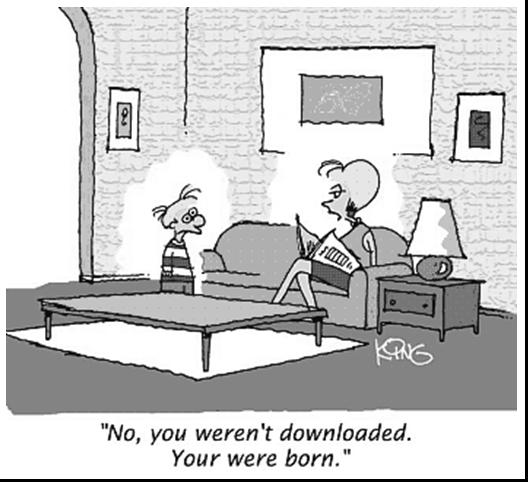
\includegraphics[width=0.4\textwidth]{./img/exemplo.jpg}\\
\small{Elaborado pelo autor.}
\end{figure}

Pode inserir várias figuras lado a lado também. Um exemplo está reproduzido a seguir.

\begin{figure}[H]
  \centering
  \caption{Canal clássico cuja obtenção da capacidade erro-zero é não-trivial.}
  \subfloat[\ ]{\label{fig:exG5}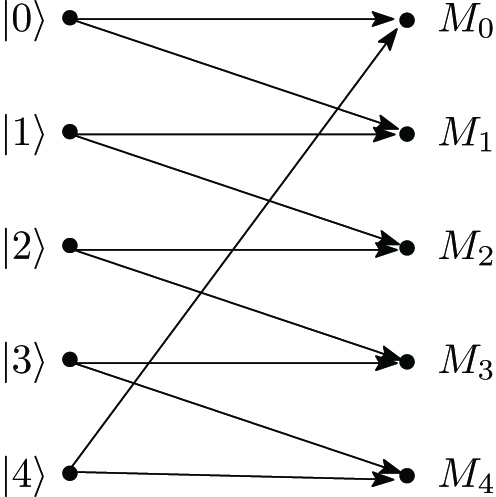
\includegraphics[width=0.3\textwidth]{./img/001}}
  \hspace{0.5cm}
  \subfloat[\ ]{\label{fig:exG52}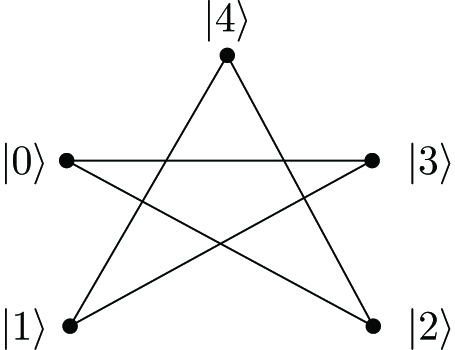
\includegraphics[width=0.3\textwidth]{./img/002}}
  \hspace{0.5cm}
  \subfloat[\ ]{\label{fig:exG53}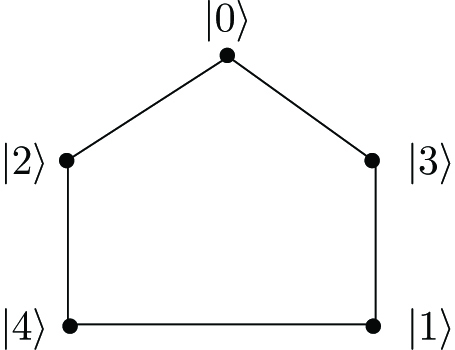
\includegraphics[width=0.3\textwidth]{./img/003}}\\
  \small{Elaborado por Bacon}
\end{figure}

\section{Referências Bibliográficas no Padrão ABNT}

Para gerar versões corretas do \textsc{Bib}\TeX das suas referências, recomenda-se usar o DOI no caso de artigos e o ISBN no caso de livros. Em posse dessas informações, consulte os seguintes links:

\begin{enumerate}
    \item \url{https://www.bibtex.com/c/doi-to-bibtex-converter/}
    \item \url{https://www.bibtex.com/c/isbn-to-bibtex-converter/}
    \item \url{http://doi-to-bibtex-converter.herokuapp.com/}
    \item \url{https://www.doi2bib.org/}
\end{enumerate}

Para saber mais sobre os tipos de referências \textsc{Bib}\TeX e seus significados, consultar a documentação oficial em \url{https://www.bibtex.com/e/entry-types/}.

Este template está integrado com o pacote \texttt{abnt2cite} que produz as referências no padrão ABNT NBR 6023.

\chapter{Título do Quarto Capítulo}


Vivamus ultricies tincidunt lacus ut pharetra. Sed fringilla hendrerit tempus. Suspendisse potenti. Cras hendrerit tortor ac est condimentum pellentesque. Morbi pretium lectus nec sapien laoreet eu malesuada diam adipiscing. Aliquam nisl ipsum, fermentum ut aliquam nec, varius sit amet nisi. Pellentesque interdum cursus malesuada. Vestibulum ante ipsum primis in faucibus orci luctus et ultrices posuere cubilia Curae; Nullam malesuada bibendum tortor, ut bibendum lorem varius eu. In eros orci, volutpat ut facilisis sit amet, commodo quis nulla.

Sed lectus metus, mollis nec vulputate id, imperdiet eget urna. Nam ut dolor at metus venenatis suscipit et in ligula. In hac habitasse platea dictumst. Mauris scelerisque dolor sed nisl mattis accumsan. Aliquam vulputate placerat feugiat. Pellentesque faucibus neque mi. Etiam porttitor varius tempus. Mauris varius porttitor posuere. Pellentesque iaculis imperdiet lobortis. Sed vulputate purus nec felis rutrum molestie.


\section{Algoritmos}




Nunc at fringilla dui. Pellentesque id tortor eu libero auctor rhoncus id vel velit. Duis auctor laoreet turpis, sed commodo tellus sollicitudin sit amet. Phasellus quis purus consectetur turpis hendrerit pretium eget in velit. Cras dignissim est vel mi malesuada a imperdiet velit condimentum. Vivamus ultrices diam non urna aliquet hendrerit. Sed lobortis, mauris quis egestas ullamcorper, nunc nulla auctor nulla, eu rutrum velit velit in nulla. Etiam lectus augue, pellentesque et porta at, pharetra id lectus. Duis eleifend eleifend mauris, nec mollis mauris vehicula nec. Nam sed ipsum ut massa lacinia vestibulum. Duis vitae sapien a lectus aliquam luctus eget sit amet nunc. Etiam a ipsum auctor tortor condimentum consectetur. Aliquam vestibulum libero sit amet nulla auctor aliquet. Sed laoreet imperdiet tellus non vulputate. Vivamus tristique ipsum vel metus venenatis in laoreet tortor hendrerit. Suspendisse potenti. Aenean tincidunt molestie libero sit amet porttitor. Class aptent taciti sociosqu ad litora torquent per conubia nostra, per inceptos himenaeos.





Cras nec quam mi, ut mattis ante. Lorem ipsum dolor sit amet, consectetur adipiscing elit. Sed fringilla auctor dictum. Nam hendrerit sapien sed massa consequat rutrum. Nullam congue, augue sed commodo malesuada, lectus nulla mollis magna, eget semper risus nisl eget elit. Duis vitae hendrerit massa. In a odio nunc, sit amet mollis dolor. In accumsan suscipit dui, a vestibulum diam condimentum ullamcorper. Etiam ut quam arcu, ac tristique ante. Vestibulum imperdiet elit non ante tristique accumsan. Donec vulputate fringilla tempor. Proin porttitor nisi nisi. Fusce vel ullamcorper orci. Lorem ipsum dolor sit amet, consectetur adipiscing elit.

Vivamus ultricies tincidunt lacus ut pharetra. Sed fringilla hendrerit tempus. Suspendisse potenti. Cras hendrerit tortor ac est condimentum pellentesque. Morbi pretium lectus nec sapien laoreet eu malesuada diam adipiscing. Aliquam nisl ipsum, fermentum ut aliquam nec, varius sit amet nisi. Pellentesque interdum cursus malesuada. Vestibulum ante ipsum primis in faucibus orci luctus et ultrices posuere cubilia Curae; Nullam malesuada bibendum tortor, ut bibendum lorem varius eu. In eros orci, volutpat ut facilisis sit amet, commodo quis nulla.




% Referência segundo o padrão ABNT
% Edite este arquivo e inclua suas referências segundo a notação do Bibtex
\bibliography{ref}



\end{document}
